%%%%%%%%%%%%
% APPENDIX %
%%%%%%%%%%%%

\clearpage
\section{Supplementary Materials - Submission Number: 14590}

\subsection{Extended results}

Addional results that complement previously shown results, are displayed in this section.

\begin{figure}[ht]
    \centering
    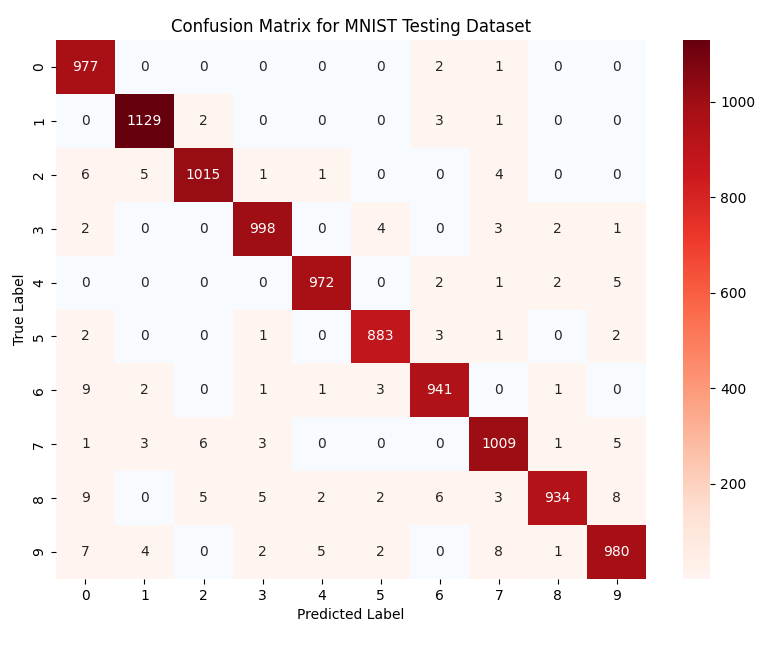
\includegraphics[width=0.99\columnwidth]{Figures/mnist_testing_confusion_matrix.png}
    \caption{Confusion matrices for the MNIST classification model on the training dataset. The matrices display the true labels on the vertical axis and the predicted labels on the horizontal axis. The diagonal elements represent correctly classified instances, while the off-diagonal elements indicate misclassifications. The corresponding confusion matrix for the testing dataset is provided in the supplementary materials.}
    \label{fig:mnist_testing_confusion_matrix}
\end{figure}

The confusion matrix for the CIFAR-10 testing dataset in Figure \ref{fig:cifar10_testing_confusion_matrix}. Examining the testing dataset, the model achieves good classification success, with perfect recognition of 'frog' class. Misclassifications are present but considerably reduced compared to the training dataset, particularly for pairs such as 'truck' and 'automobile', as well as 'cat' and 'dog'. The reduced confusion in the test set is also reflected in the softmax distance to cluster centroid.

\begin{figure}[ht]
    \centering   
    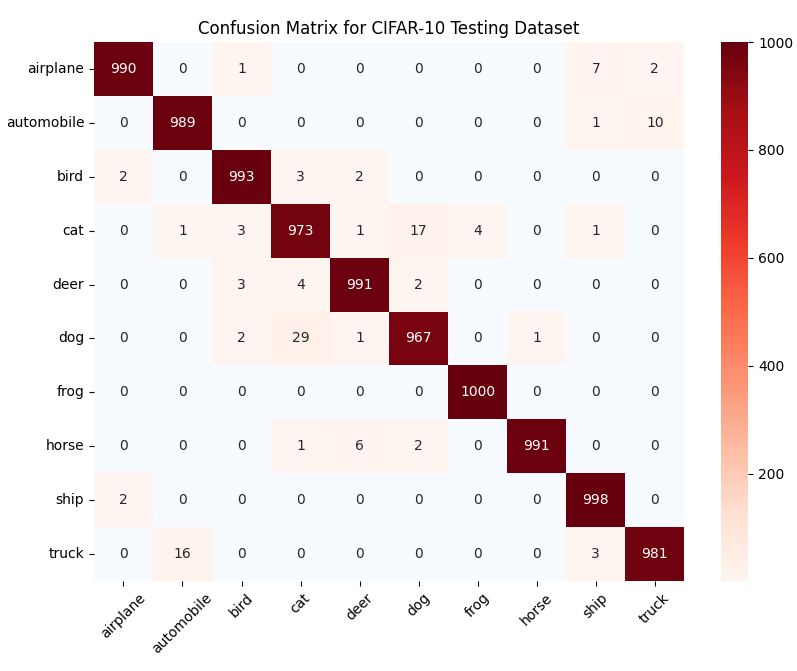
\includegraphics[width=0.99\columnwidth]{Figures/cifar10_testing_confusion_matrix.png}
    \caption{Confusion matrix for the CIFAR-10 classifier model training dataset dataset dataset correct and incorrect classifications. The corresponding matrix for the testing dataset is given in the supplementary materials.}
    \label{fig:cifar10_testing_confusion_matrix}
\end{figure}

%%%%%%%%%%%%%%%%%%%%%%%%%%%%%%%%%%%%%%%%%%%
% COMBINED CIFAR10 MNIST ACCURACY VS MEAN %
% CLASS PREDICTION DISTANCE TO CENTROID   %
%%%%%%%%%%%%%%%%%%%%%%%%%%%%%%%%%%%%%%%%%%%

Figures \ref{fig:CIFAR10_plot_accuracy_vs_distance_linear_fit} and \ref{fig:mnist_plot_accuracy_vs_distance_linear_fit} suggest how both the trained CNN and ViT models achieves higher predictive accuracy for classes that have lower softmax distance to their respective class centroids, compared to classes for which the models obtain lower predictive accuracy.

% In the context of the MNIST dataset, the derived linear functions from the training and testing data exhibit a negative correlation between the classification accuracy and the mean class distances to the centroids. Specifically, the training data is described by the function $ y = -0.806x + 1.009 $, and the testing data by $ y = -0.677x + 1.004 $. The negative coefficients of the linear terms $ -0.806 $ and $ -0.677 $, respectively) indicate that an increase in the mean distance to the centroid correlates with a decrease in classification accuracy for both datasets.

The scatter plots show the relationship between classification accuracy and mean class distance to the centroid for the CIFAR-10 MNIST dataset. Training data (blue dots) and testing data (green dots) are each fitted with a linear regression line, demonstrating a negative correlation where increased mean distance corresponds to decreased accuracy. For the CNN/MNIST experiment, the steeper slope of the training data fit (-0.806) compared to the testing data fit (-0.677) reflects the greater accuracy and more compact cluster obtained from the correct test predictions compared to the cluster obtained from correct training predictions, noting that both training and testing data use centroids obtained from the correctly classified examples in the training dataset.

These results show an inverse relationship: as the mean distance from the data points in a class to their centroid increases, the propensity for correct classification diminishes. This could be due to the spread of data points within a class – greater distances from the centroid reflect a larger variance within the class, potentially making it more challenging for the classifier to identify the defining characteristics of each class accurately.

The CIFAR-10 linear fit is steeper as can be observed by the y axis values, although it can be argued provides a better fit.

% Plot created manually from MNIST and CIFAR10 plots created by function plot_accuracy_vs_distance_linear_fit
\begin{figure*}[ht]
    \centering
    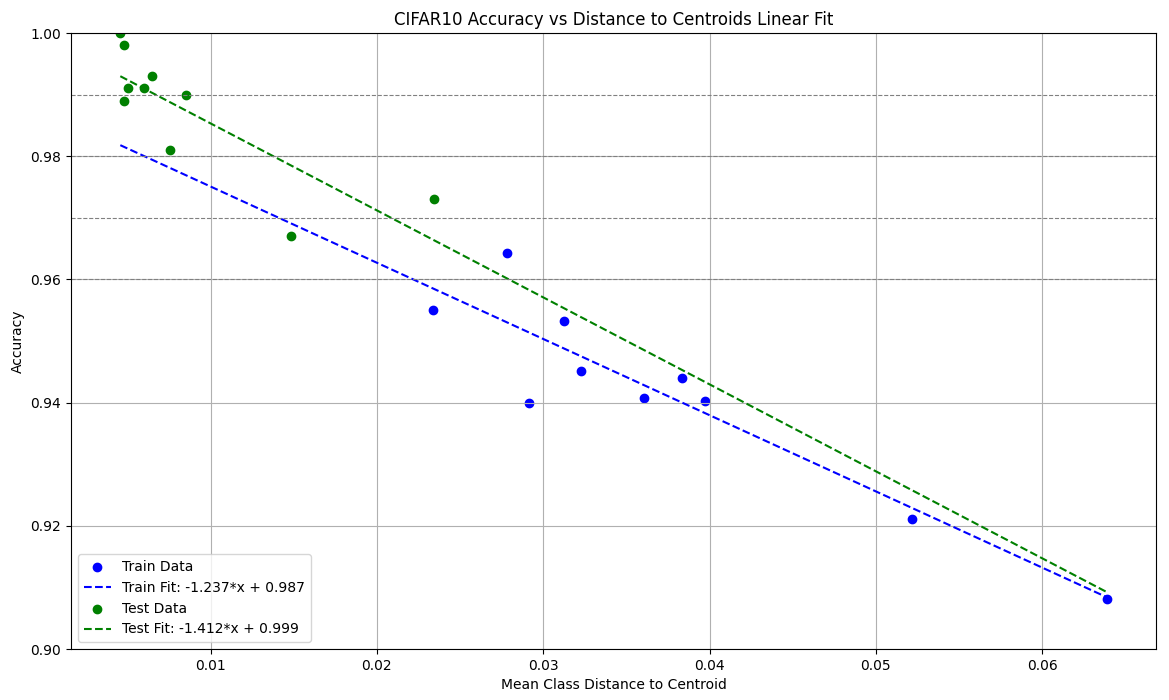
\includegraphics[width=0.99\textwidth]{Figures/CIFAR10_plot_accuracy_vs_distance_linear_fit.png}
    \caption{Expected accuracy linear fit based on prediction softmax distance to class centroid. ViT/CIFAR-10 training dataset predictions}
\label{fig:CIFAR10_plot_accuracy_vs_distance_linear_fit}
\end{figure*}

\begin{figure*}[ht]
    \centering
    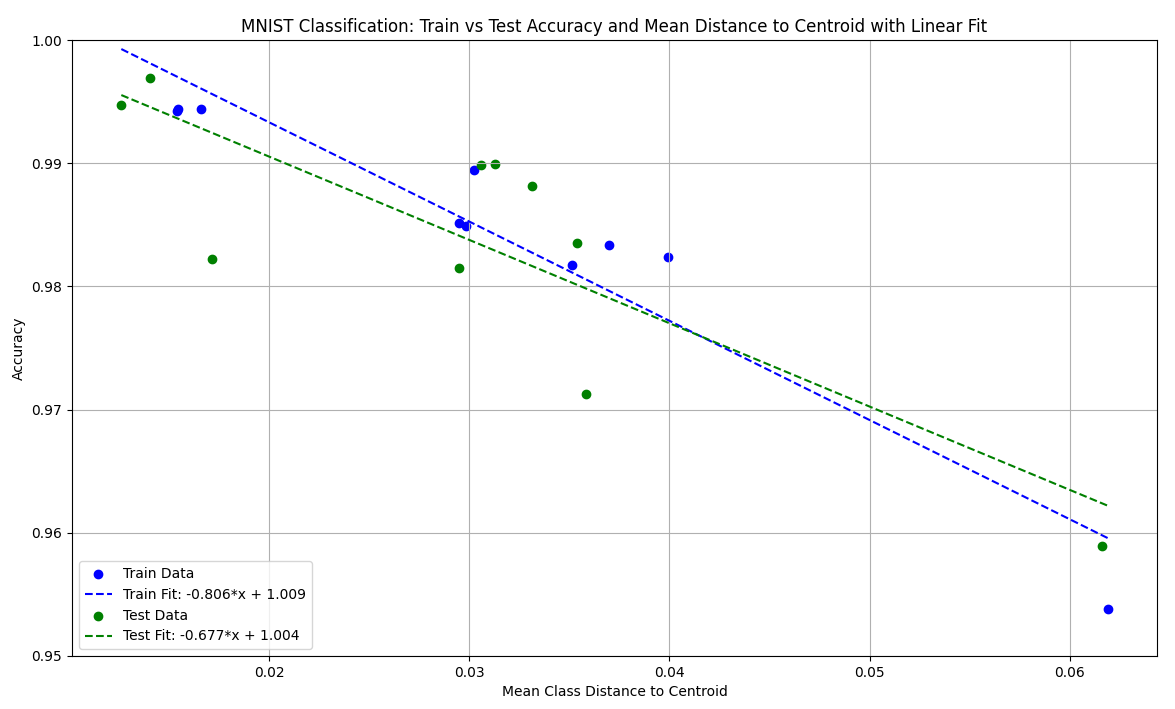
\includegraphics[width=0.99\textwidth]{Figures/mnist_plot_accuracy_vs_distance_linear_fit.png}
    \caption{Expected accuracy linear fit based on prediction softmax distance to class centroid. CNN/MNIST training dataset predictions.}
\label{fig:mnist_plot_accuracy_vs_distance_linear_fit}
\end{figure*}

%Combined_CIFAR10_MNIST_Classification_Train_Test_Accuracy_Mean_Distance_to_Centroid_Linear_Fit.png

% \subsection{Overlap table CIFAR discussion 2}

% %%%%%%%%%%%%%%%
% % LATEX TABLE %
% %%%%%%%%%%%%%%%

% % Table generated by function call
% % centroid_distance_overlap_latex(d2c_train_correct, 
% %                                 d2c_train_incorrect, 
% %                                 d2c_test_correct, 
% %                                 d2c_test_incorrect, 
% %                                 labels=class_labels,
% %                                 caption='CIFAR10 centroid distances overlap count for correct predictions above incorrect threshold'
% %                             ) 

% \begin{table}[htbp]
% \centering
% \begin{tabular}{|c|c|c|c|c|c|c|}
% \hline
% Class & \multicolumn{3}{c|}{Train Data - Train Centroids} & \multicolumn{3}{c|}{Test Data - Train Centroids} \\
% \hline
%  & Count & Total & Overlap & Count & Total & Overlap \\
% \hline
% plane & 13 & 4252 & 0.31\% & 1 & 990 & 0.10\% \\
% auto & 1 & 4326 & 0.02\% & 0 & 989 & 0.00\% \\
% bird & 9 & 4216 & 0.21\% & 0 & 993 & 0.00\% \\
% cat & 20 & 4103 & 0.49\% & 2 & 973 & 0.21\% \\
% deer & 14 & 4255 & 0.33\% & 0 & 991 & 0.00\% \\
% dog & 11 & 4157 & 0.26\% & 1 & 967 & 0.10\% \\
% frog & 11 & 4310 & 0.26\% & 0 & 1000 & 0.00\% \\
% horse & 12 & 4223 & 0.28\% & 0 & 991 & 0.00\% \\
% ship & 11 & 4258 & 0.26\% & 0 & 998 & 0.00\% \\
% truck & 10 & 4251 & 0.24\% & 0 & 981 & 0.00\% \\
% \hline
% Totals & 112 & 42351 & 0.26\% & 4 & 9873 & 0.04\% \\
% \hline
% \end{tabular}
% \caption{CIFAR10 centroid distances overlap count for correct predictions above incorrect threshold}
% \label{tab:centroid_distance_overlap}
% \end{table}

\begin{table*}[htbp]
\centering
\begin{tabular}{|c|c|c|c|c|c|c|}
\hline
Digit & \multicolumn{3}{c|}{Train Data - Train Centroids} & \multicolumn{3}{c|}{Test Data - Train Centroids} \\
\hline
 & Count & Total & Overlap & Count & Total & Overlap \\
\hline
0 & 2 & 5890 & 0.03\% & 1 & 977 & 0.10\% \\
1 & 0 & 6704 & 0.00\% & 0 & 1129 & 0.00\% \\
2 & 1 & 5859 & 0.02\% & 0 & 1015 & 0.00\% \\
3 & 3 & 6019 & 0.05\% & 1 & 998 & 0.10\% \\
4 & 0 & 5755 & 0.00\% & 0 & 972 & 0.00\% \\
5 & 5 & 5339 & 0.09\% & 0 & 883 & 0.00\% \\
6 & 2 & 5884 & 0.03\% & 1 & 941 & 0.11\% \\
7 & 2 & 6199 & 0.03\% & 0 & 1009 & 0.00\% \\
8 & 12 & 5581 & 0.22\% & 1 & 934 & 0.11\% \\
9 & 1 & 5844 & 0.02\% & 0 & 980 & 0.00\% \\
\hline
Totals & 28 & 59074 & 0.05\% & 4 & 9838 & 0.04\% \\
\hline
\end{tabular}
\caption{MNIST counts of correctly classified training and testing image predictions and counts with distance to centroids equal or above error threshold.}
\label{tab:centroid_distance_overlap_mnist}
\end{table*}

\begin{table*}[htbp]
\centering
\begin{tabular}{|c|c|c|c|c|c|c|}
\hline
Class & \multicolumn{3}{c|}{Train Data - Train Centroids} & \multicolumn{3}{c|}{Test Data - Train Centroids} \\
\hline
 & Count & Total & Overlap & Count & Total & Overlap \\
\hline
plane & 13 & 4252 & 0.31\% & 1 & 990 & 0.10\% \\
auto & 1 & 4326 & 0.02\% & 0 & 989 & 0.00\% \\
bird & 9 & 4216 & 0.21\% & 0 & 993 & 0.00\% \\
cat & 20 & 4103 & 0.49\% & 2 & 973 & 0.21\% \\
deer & 14 & 4255 & 0.33\% & 0 & 991 & 0.00\% \\
dog & 11 & 4157 & 0.26\% & 1 & 967 & 0.10\% \\
frog & 11 & 4310 & 0.26\% & 0 & 1000 & 0.00\% \\
horse & 12 & 4223 & 0.28\% & 0 & 991 & 0.00\% \\
ship & 11 & 4258 & 0.26\% & 0 & 998 & 0.00\% \\
truck & 10 & 4251 & 0.24\% & 0 & 981 & 0.00\% \\
\hline
Totals & 112 & 42351 & 0.26\% & 4 & 9873 & 0.04\% \\
\hline
\end{tabular}
\caption{CIFAR10 counts of correctly classified training and testing image predictions and counts with distance to centroids equal or above error threshold.}
\label{tab:centroid_distance_overlap}
\end{table*}

Table \ref{tab:centroid_distance_overlap_mnist} presents an analysis of the counts and percentages of correctly classified images in the training and testing datasets that have softmax distances to their respective class centroids above a certain threshold. The threshold is determined by the nearest softmax distance to the centroid for the incorrectly classified classes.

The table is divided into two main sections: "Train Data - Train Centroids" and "Test Data - Train Centroids." For each section, the table provides the count of images that satisfy the threshold condition, the total number of images in each class, and the percentage of overlap (i.e., the proportion of images above the threshold relative to the total count).

Looking at the "Train Data - Train Centroids" section, we observe that the overlap percentages are relatively low, ranging from 0.00\% to 0.22\%. This suggests that only a small fraction of the correctly classified training images have softmax distances to their centroids above the threshold set by the incorrectly classified images. The highest overlap is observed for digit class 8, with 12 out of 5,581 images (0.22\%) having distances above the threshold.

Similarly, in the "Test Data - Train Centroids" section, the overlap percentages are even lower, ranging from 0.00\% to 0.11\%. This indicates that the trained model is able to correctly classify the majority of the test images while maintaining a distance to the centroids below the threshold set by the incorrectly classified images. The highest overlap in the test data is observed for digit classes 6 and 8, with 1 out of 941 (0.11\%) and 1 out of 934 (0.11\%) images, respectively, having distances above the threshold.

The Totals summarise the overall counts and overlap percentages across all digit classes. For the training data, 28 out of 59,074 images (0.05\%) have distances above the threshold, while for the test data, only 4 out of 9,838 images (0.04\%) exceed the threshold.

The low overlap percentages indicate that the majority of the correctly classified images are well-separated from the incorrectly classified images in terms of their softmax distances to the centroids. This analysis provides insights into the softmax distance being a proxy to distinguish between between correct and incorrect digit classifications based on the proximity of the images to their respective class centroids in the softmax distance space. The same analysis applies to Table \ref{tab:centroid_distance_overlap}. Most indicative of the consistency of the suggested approach is than both CIFAR-10 and MNIST present an overlap of 0.04\% for correctly classified images at or above threshold. Note we tag the images in the overlap as incorrectly classified, for the sake of assuring that all softmax distances to cluster centroid below threshold are correct classifications.

\begin{figure*}[ht]
    \centering
    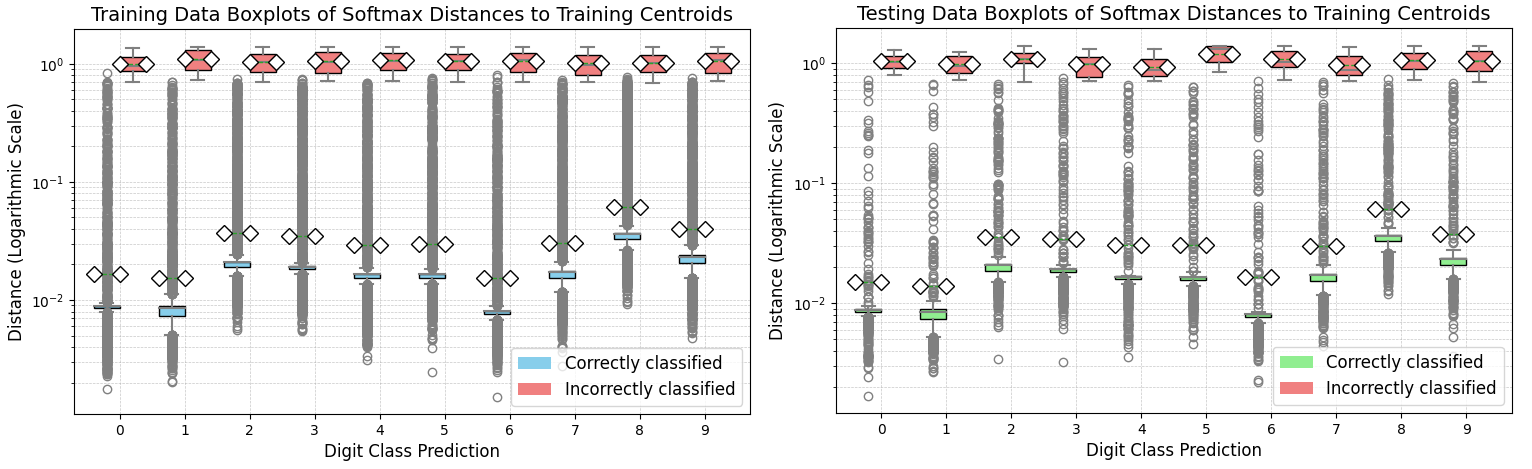
\includegraphics[width=0.99\textwidth]{Figures/MNIST_boxplots_side_by_side_x2.png}   \captionsetup{justification=raggedright,singlelinecheck=false}
    \caption{Distribution of Distances to Centroids for Correctly and Incorrectly Classified Instances in Training and Testing MNIST data, where training data is on the left and testing data is displayed on the right. Distances on y axis are shown on a logarithmic scale. Centroids are obtained from correctly classified training examples, then used for both training and testing datasets, a cluster is not created from the testing softmax distances. }
    \label{fig:MNIST_boxplots_side_by_side_x2}
\end{figure*}

% AVERAGE SOFTMAX OUTPUTS CNN/MNIST, ViT/CIFAR-10, training and testing datasets

% function call
% plot_digit_averages(test_correct_predictions, test_incorrect_predictions, color1='lightgreen', color2='lightcoral', data="Testing Data")
\begin{figure*}[ht]
    \centering
    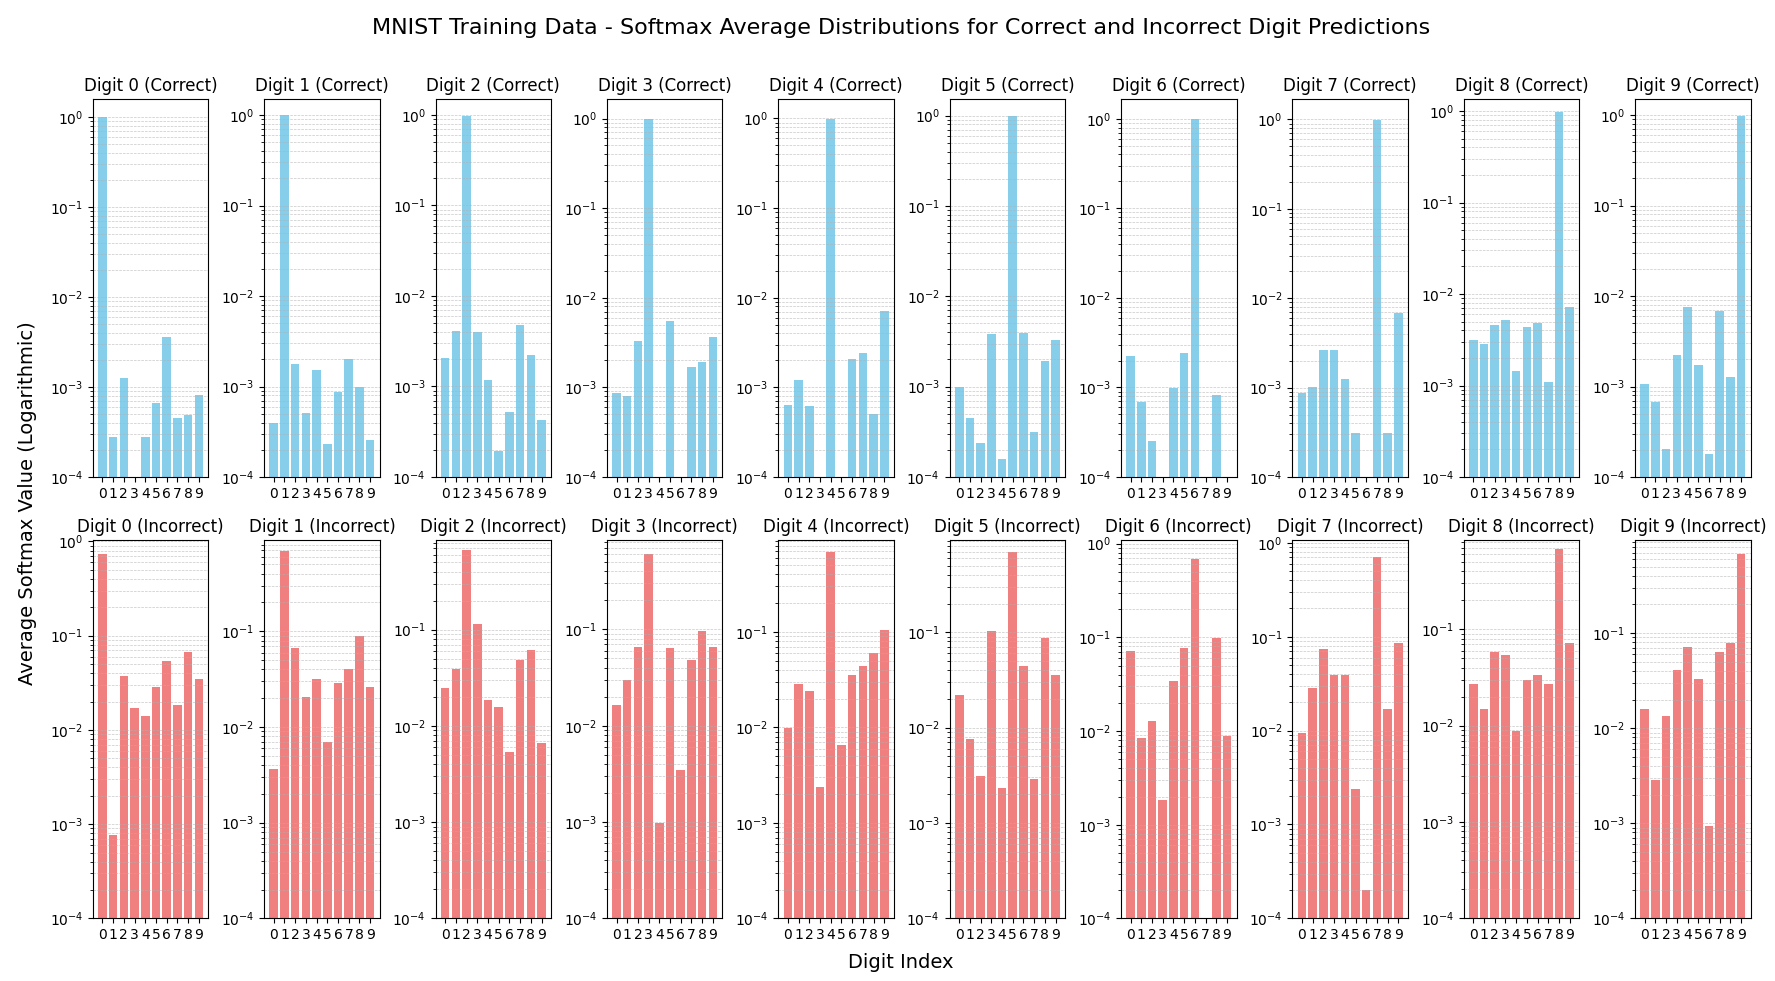
\includegraphics[width=0.99\textwidth]{Figures/MNIST_Softmax_Averages_Training.png}
    \caption{Average Softmax Probabilities for Correctly and Incorrectly Classified Digits in the MNIST Testing Dataset.}
    \label{fig:MNIST_Softmax_Averages_Training}
\end{figure*}

Figure \ref{fig:MNIST_Softmax_Averages_Training} shows the average softmax probabilities for each digit class (0 to 9) in the MNIST training dataset, separated into correctly classified instances (top row) and incorrectly classified instances (bottom row). The probabilities are displayed on a logarithmic scale. For correctly classified digits, the highest average probability is observed for the corresponding true digit class, indicating strong confidence in the correct predictions. In contrast, for incorrectly classified digits, the average probabilities are more evenly distributed across different digit classes, suggesting lower confidence and potential confusion between similar-looking digits.
Figure \ref{fig:MNIST_Softmax_Averages_Testing} is the corresponding plot for the MNIST testing dataset.

% function call
% plot_digit_averages(test_correct_predictions, test_incorrect_predictions, color1='lightgreen', color2='lightcoral', data="Testing Data")
\begin{figure}[ht]
    \centering
    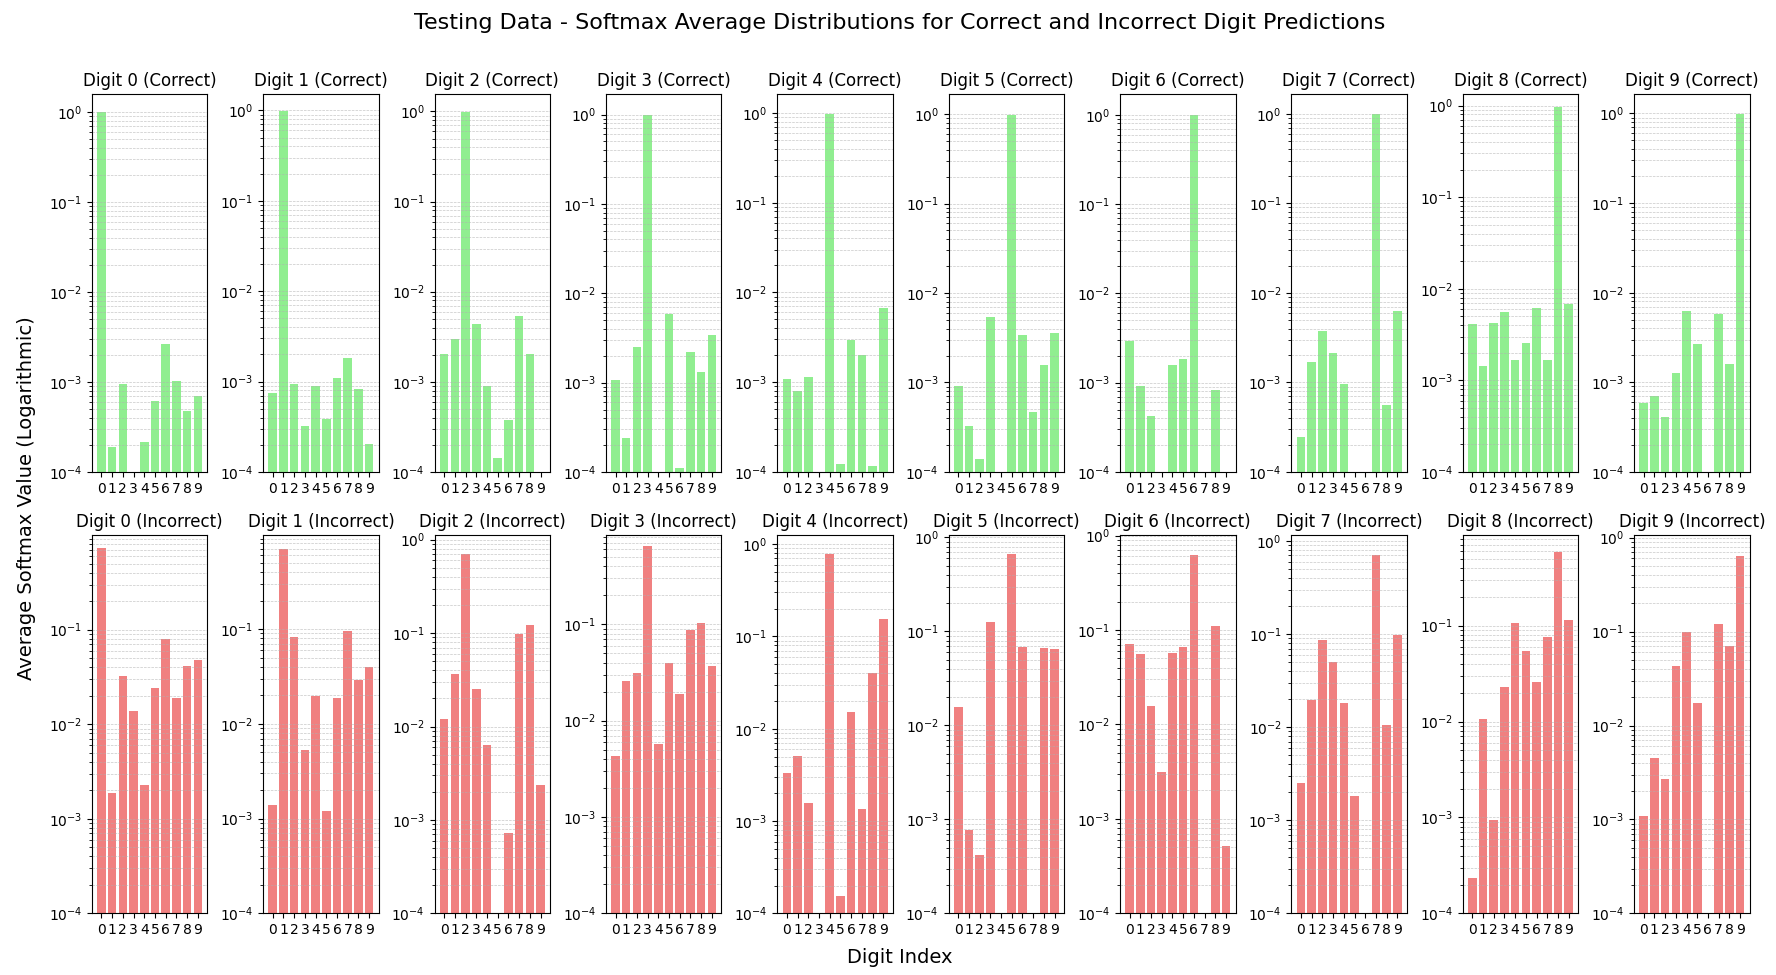
\includegraphics[width=0.99\textwidth]{Figures/MNIST_Softmax_Averages_Testing.png}
    \caption{Average Softmax Probabilities for Correctly and Incorrectly Classified Digits in the MNIST Testing Dataset.}
    \label{fig:MNIST_Softmax_Averages_Testing}
\end{figure}


\begin{figure}[ht]
    \centering
    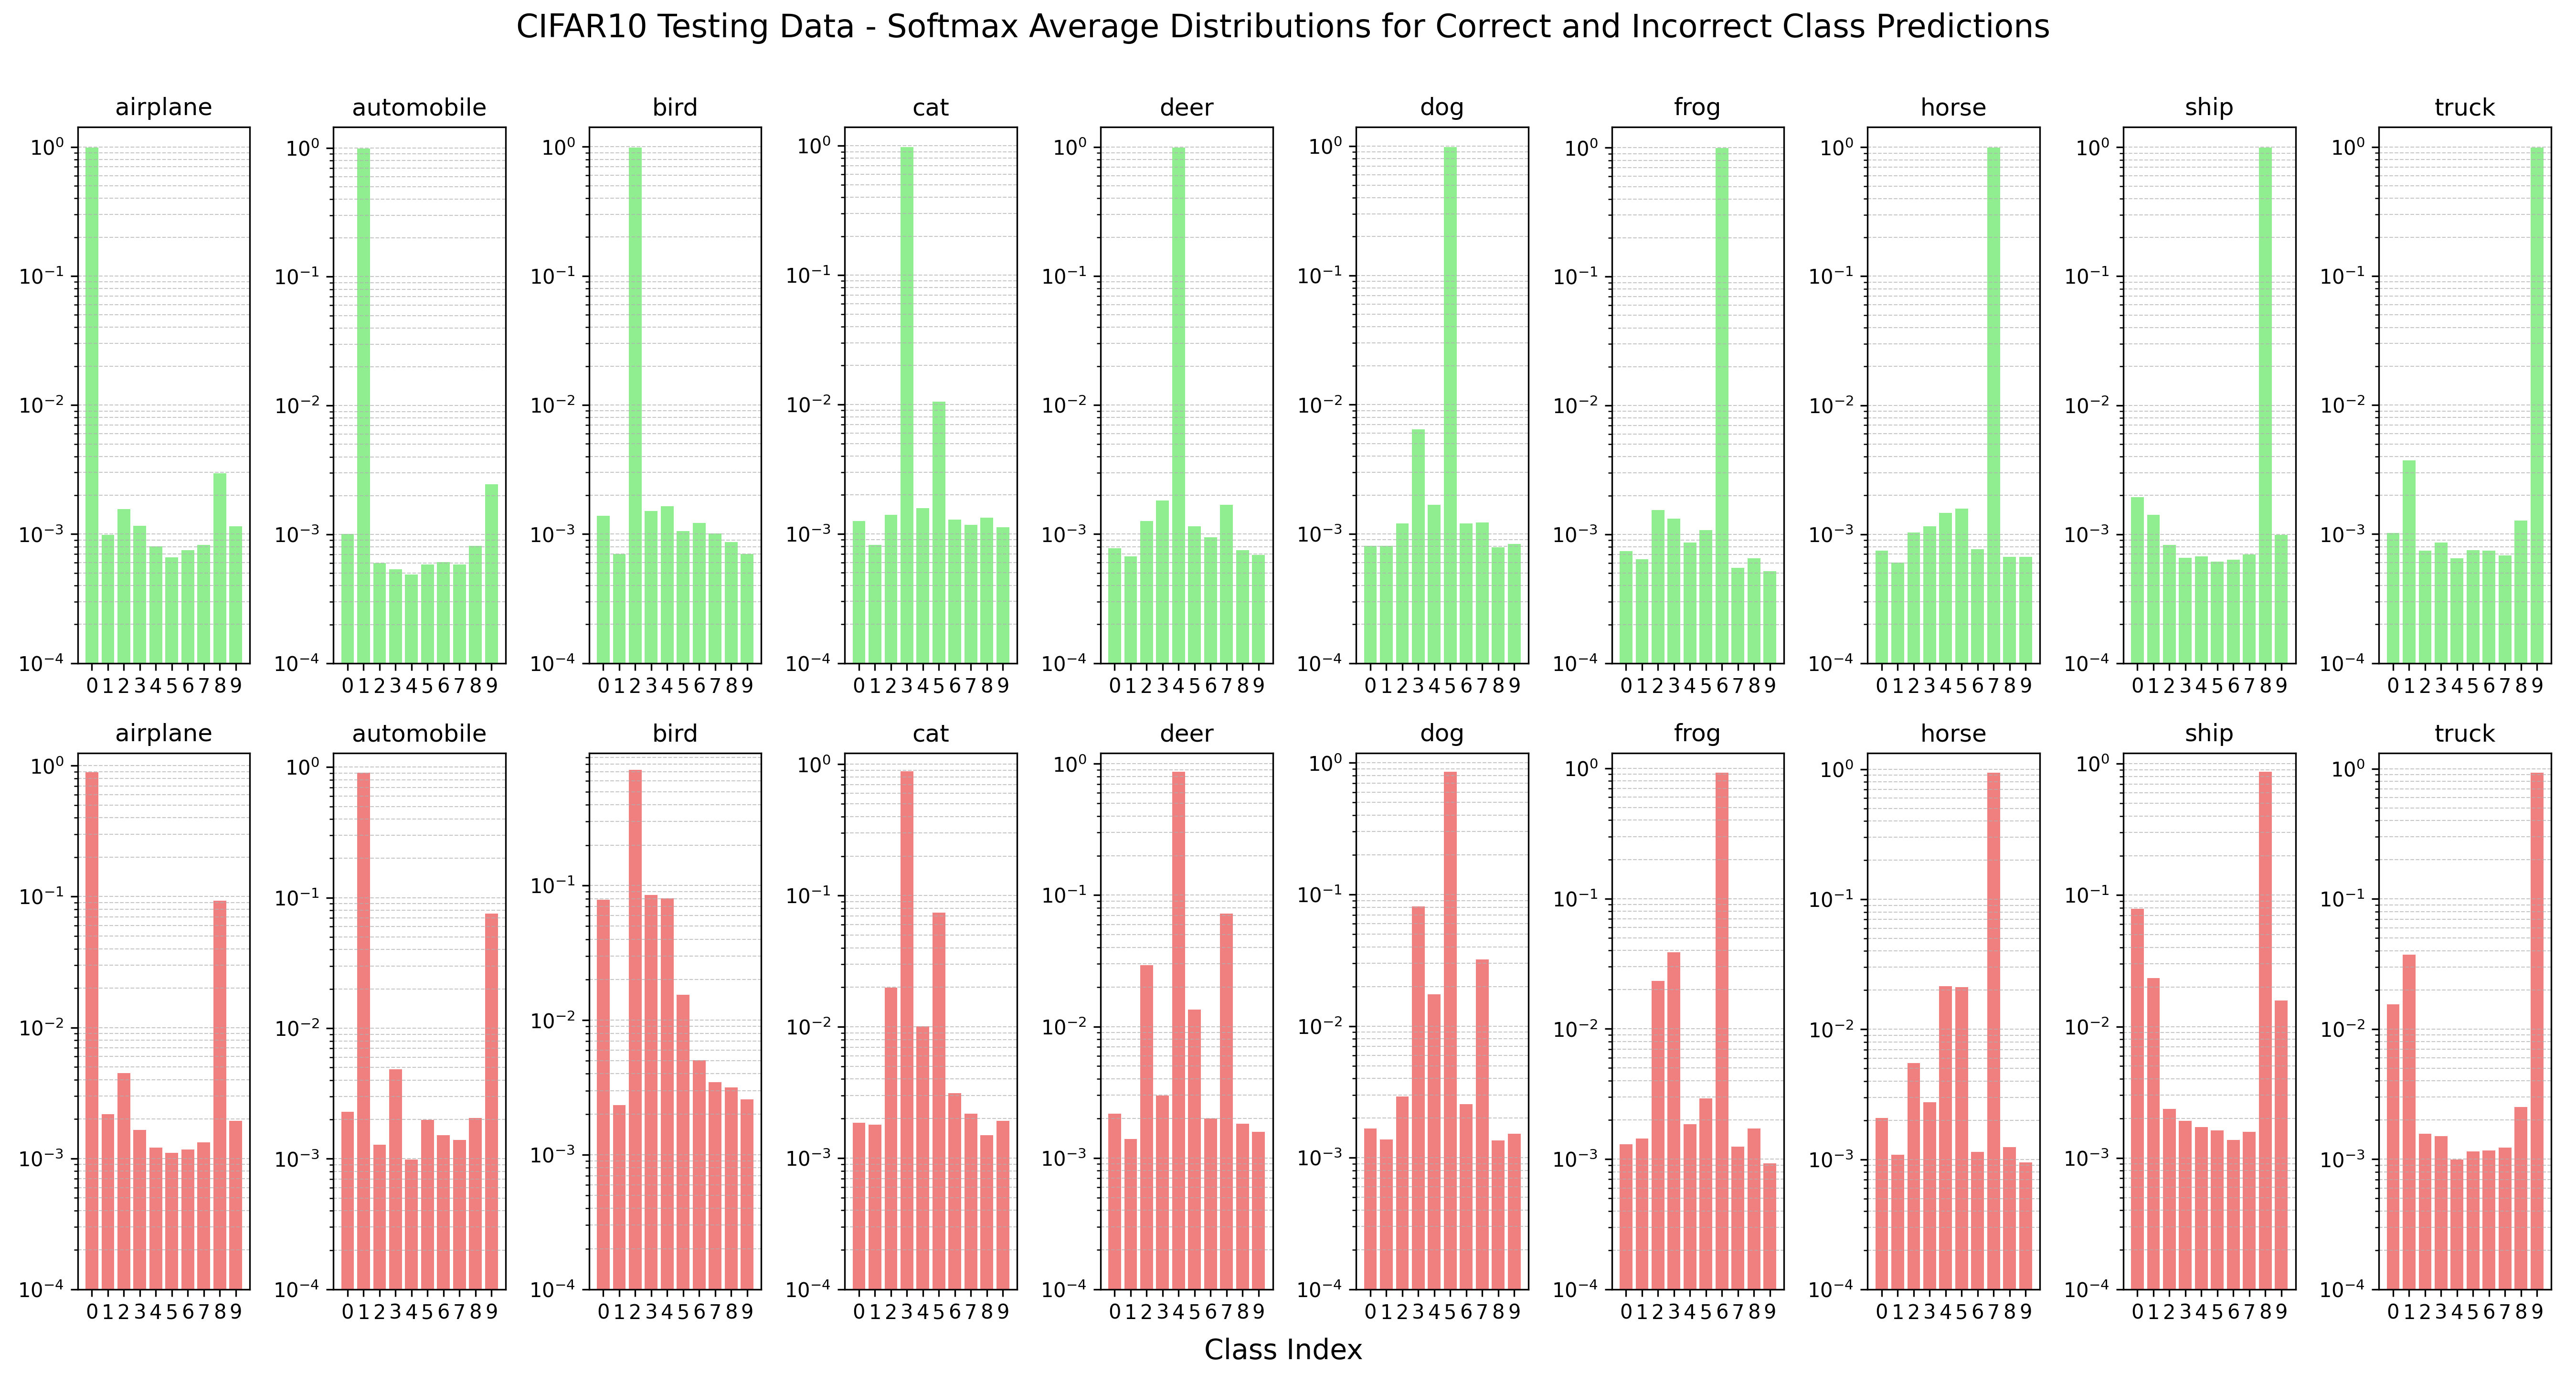
\includegraphics[width=0.99\textwidth]{Figures/CIFAR10_testing_plot_centroid_distance_bars.png}
    \caption{Please zoom in for detail. Average Softmax Probabilities for Correctly and Incorrectly Classified classes in the CIFAR-10 Testing Dataset}
    \label{fig:CIFAR10_testing_plot_centroid_distance_bars.png}
\end{figure}

%%%%%%%%%%%%%%%%%%%%%%%%%%%%%%%%%%%%%%%%%%%
% COMBINED CIFAR10 MNIST ACCURACY VS MEAN %
% CLASS PREDICTION DISTANCE TO THRESHOLD  %
%%%%%%%%%%%%%%%%%%%%%%%%%%%%%%%%%%%%%%%%%%%

% Plot created by joining plots created by plot_accuracy_vs_distance_linear_fit

\begin{figure*}[ht]
    \centering
    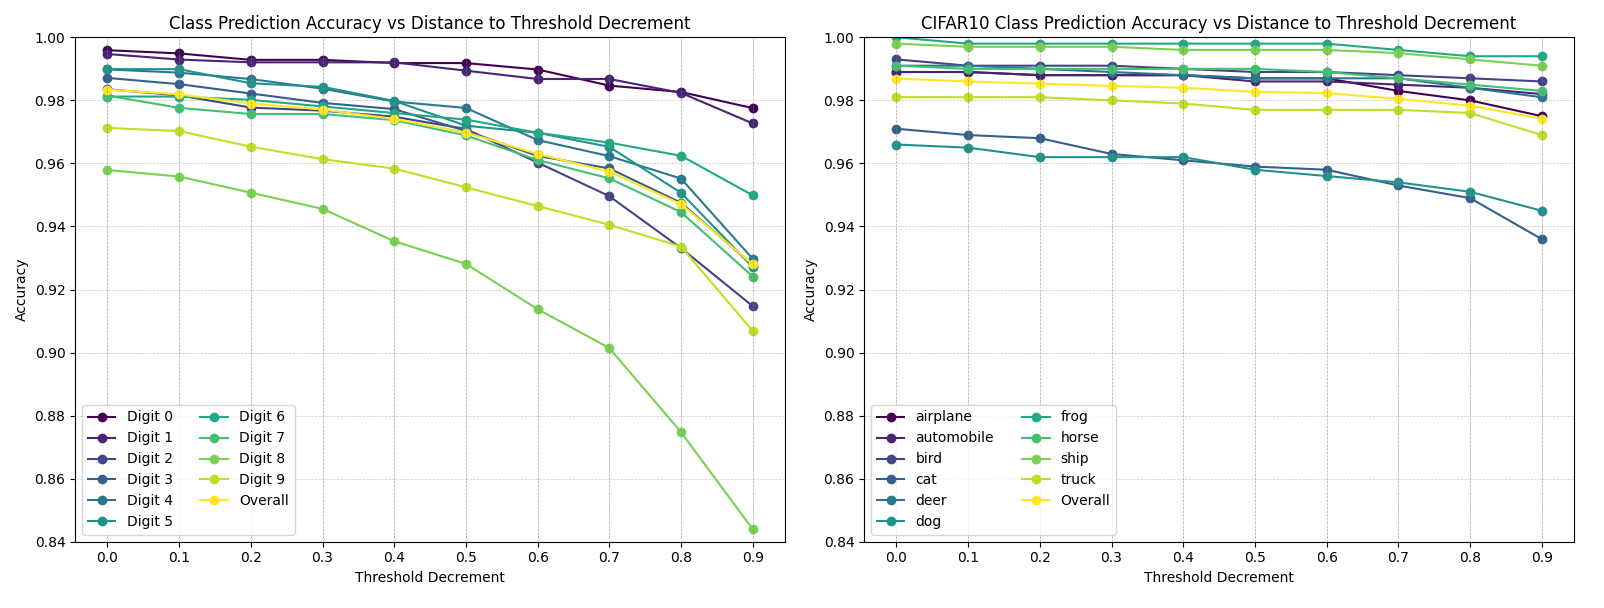
\includegraphics[width=0.99\textwidth]{Figures/Combined_CIFAR10_MNIST_single_plot_accuracy_decrements.png}
    \caption{Expected accuracy decrease as a result of threshold decrease. MNIST data is on the left, CIFAR-10 is on the right. The x axis shows the threshold decrement in factors of 0.1, that is, at 0.1 the threshold is 90\% of the original threshold while at 0.9 the threshold is 10\% of the original threshold and consequently neared to the class centroid.}
\label{fig:Combined_CIFAR10_MNIST_single_plot_accuracy_decrements.png}
\end{figure*}